In section \ref{sec:elasticity} we outlined a discretization using a single quadrature point per cell. This choice promises better performance since it requires only one SVD/polar decomposition per cell (rather than 8 with Gauss quadrature). Unfortunately, this leads to catastrophic defects if used without modification. Our method stabilizes the one point quadrature approach and thus drastically improves performance by requiring just one SVD/polar decomposition per cell.

Consider that a cell has 8 points (24 DOFs), but the one-point quadrature based elemental energy is only dependent on the cell-centered deformation gradient (9 DOFs), leading to a large subspace of deformation modes that have no effect on the discrete energy. If we were
fortunate, this ``nullspace'' might only appear element-by-element and in the
union of all elements, these modes would be penalized. Unfortunately, in our
case, there exist non-physical global modes that have no effect on discrete
energy. For example, consider a red-black ordering of the grid nodes, and assign one
constant displacement to red nodes and another to all black ones. This is not
seen by the discrete energy and is visible as parasitic ``hourglassing''
artifacts in force equilibrium (as in figure~\ref{fig_instability}).  These
oscillatory nullspace modes are more than visual artifacts, they compromise the
ellipticity of the discrete equations in multigrid methods. This is why standard
discretizations use higher-order quadrature, gaining stability at higher cost.

\begin{figure}[tbh]
\center{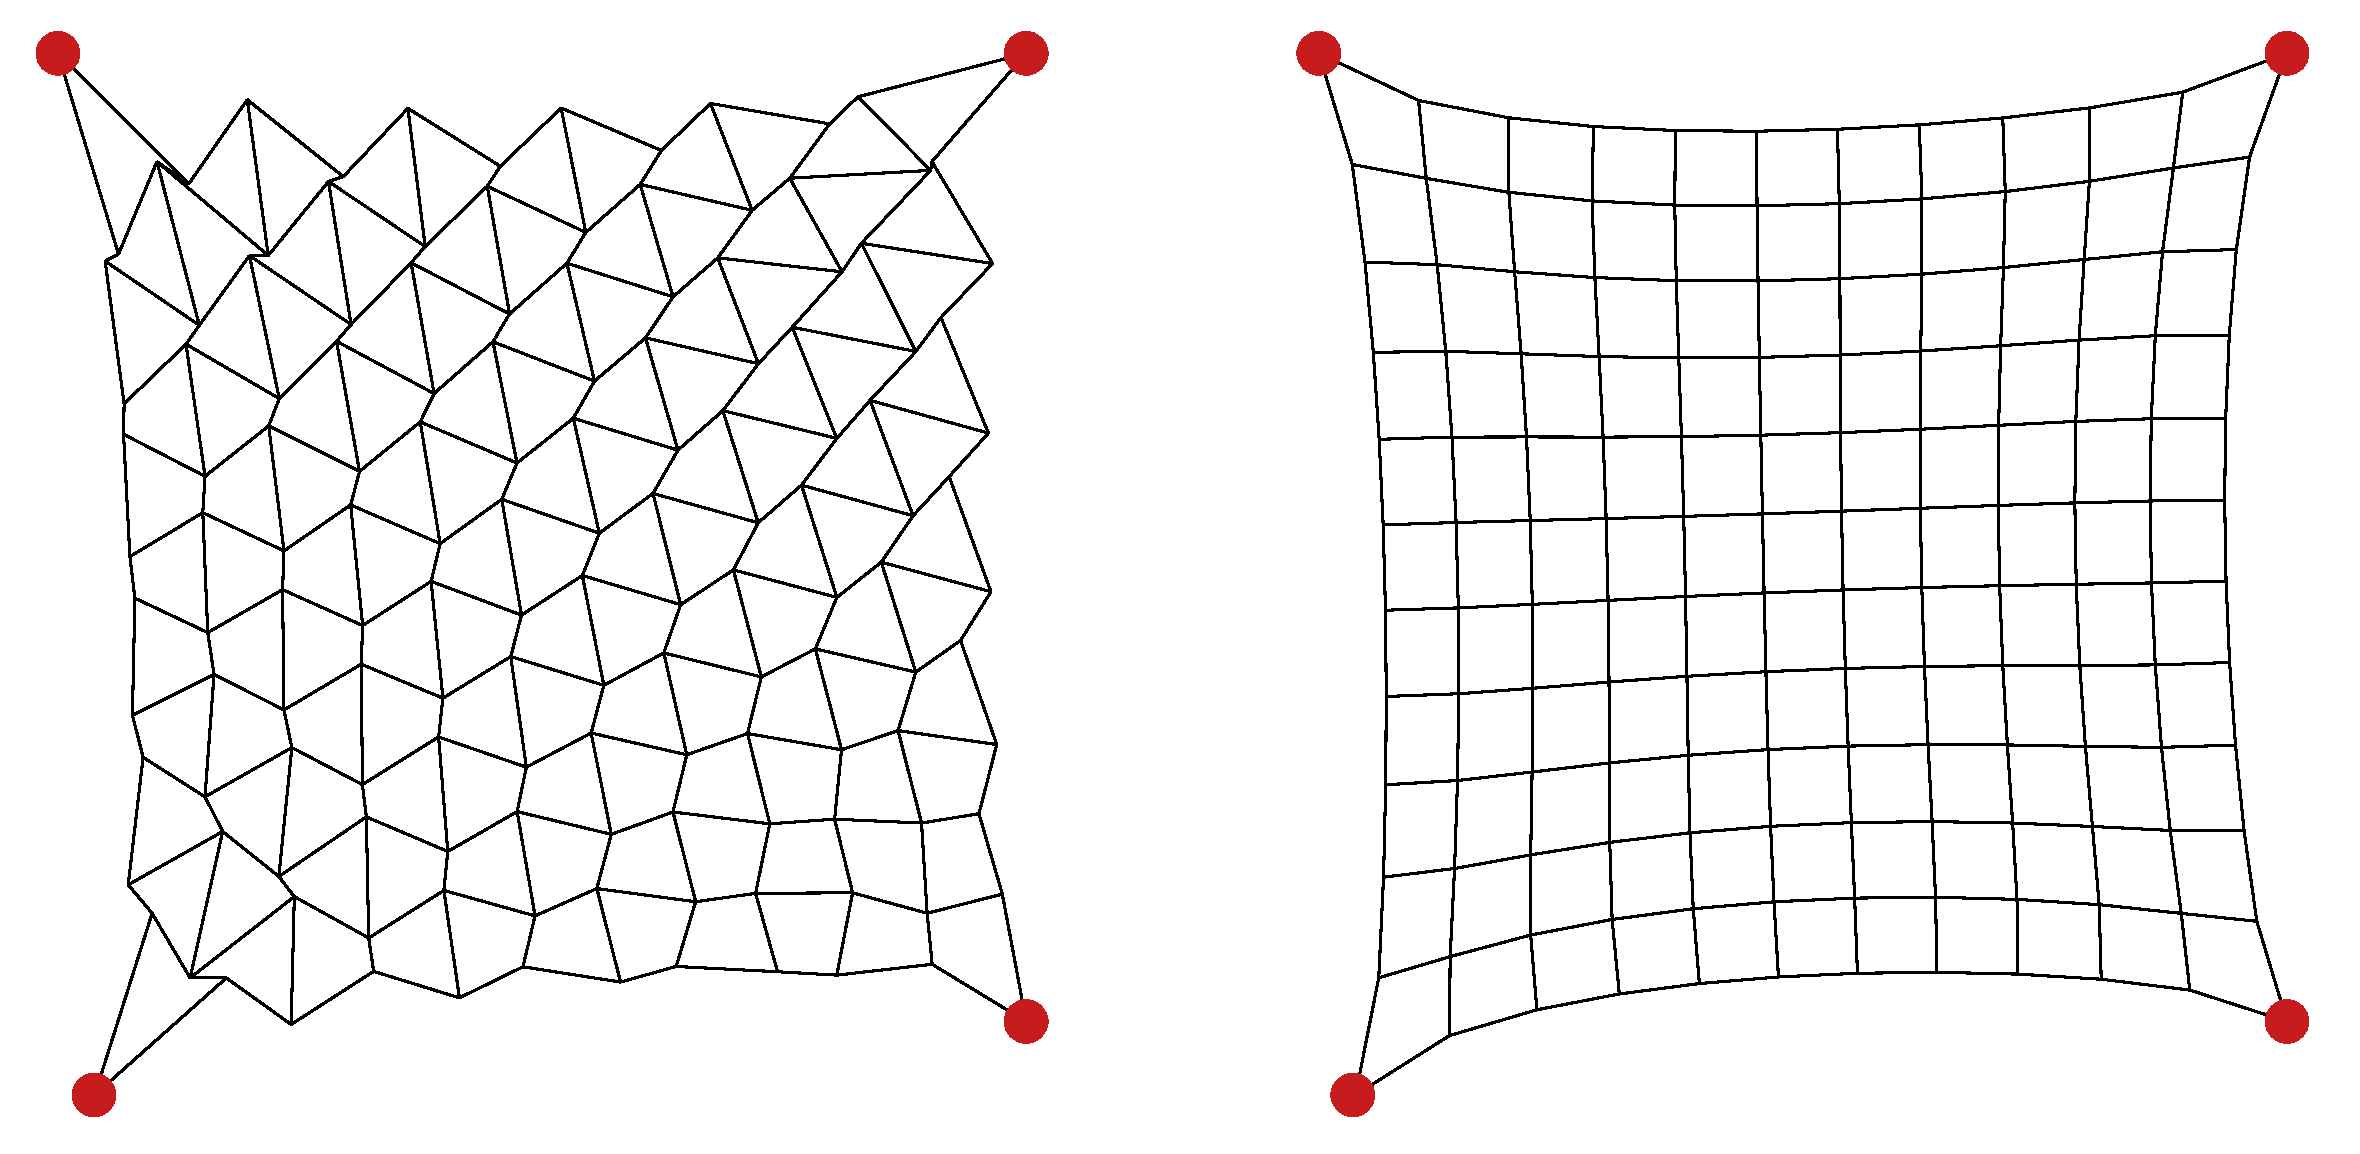
\includegraphics[width=.6\columnwidth]{elasticity/figures/discretization}}
\caption[A 2D comparison of quadrature rules]{A 2D elastic patch is stretched by pinning the four corners to target locations. Left: The unmodified one-point quadrature method is riddled by hourglassing
  instabilities. Right: Our method.}
\vspace{-10pt}
\label{fig_instability}
\end{figure}


\begin{figure}[th]
\centering
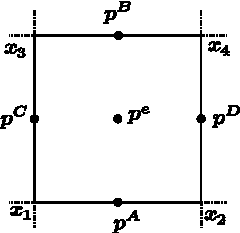
\includegraphics[width=.3\columnwidth]{elasticity/figures/quadrature}
\caption{Our quadrature}
\label{fig_quadrature}
\end{figure}
We remedy this instability by proposing a new integration rule that is
stable yet computationally cheap (requires only one polar decomposition per cell). As an initial observation, we have experimentally verified that the term $\mu\|\mathbf{F}-\mathbf{R}\|_F^2$ in equation (\ref{eqn_energy_F}) is
the one which primarily determines stability; we observed that if a stable technique (e.g.\ 8-point Gauss quadrature) is used to integrate this term, the entire scheme will remain
stable, even if the naive 1-point quadrature is used for the term  $\frac{\lambda}{2}\tr^2(\mathbf{R}^T\mathbf{F}-\mathbf{I})$. Thus, we will initially present our approach in the context
of the simpler energy $\Psi=\mu\|\mathbf{F}-\mathbf{R}\|_F^2$, and address the 2D case first (e.g.\ on a square lattice). In addition to the cell center $\vec{p}^e$ we introduce four
additional quadrature points $\vec{p}^q,\ q\in\{A,B,C,D\}$, located on
edge centers of the quadrilateral lattice, as seen in figure
(\ref{fig_quadrature}). We write the energy density as
\begin{equation}
\Psi=\mu\sum_{i,j}
  (F_{ij}-R_{ij})^2.
\label{eqn_energy_only_mu}
\end{equation}
Our approach will essentially follow a different quadrature rule for every term $(F_{ij}-R_{ij})^2$ in this expression. In particular, instead of using the single quadrature point
$\vec{p}^e$ at the cell center, we will use those locations within the cell (possibly more than one) where $F_{ij}$ is ``naturally'' defined, as a central difference of just two degrees
of freedom. In this way, we avoid the averaging and risk of cancellation associated with expressing all derivatives exclusively at the cell center. From figure \ref{fig_quadrature} we
observe that the $x$-derivatives $F_{11}$ and $F_{21}$ are naturally defined at the centers $\vec{p}^A,\vec{p}^B$ of $x$-oriented edges, while the $y$-derivatives $F_{12}$ and $F_{22}$
are naturally located at points $\vec{p}^C$ and $\vec{p}^D$. We also evaluate the cell-centered deformation gradient $\mathbf{F}^e$ once more, following exactly equation
(\ref{eqn_discrete_gradient}) as before. We compute matrix $\mathbf{R}^e$ from the Polar decomposition of $\mathbf{F}^e$, and use the information from this matrix wherever $R_{ij}$ is needed 
in equation (\ref{eqn_energy_only_mu}). Finally, our proposed quadrature method takes the form:
\begin{equation}
\!E_e=\frac{\mu h^2}{2}\sum_{i=1}^2\left[\sum_{q\in\{A,B\}}\!\!\!\!\left(F_{i1}^q\!-\!R_{i1}^e\right)^2+\!\!\!\!\sum_{q\in\{C,D\}}\!\!\!\!\left(F_{i2}^q\!-\!R_{i2}^e\right)^2\right].
\label{eqn_quadrature}
\end{equation}
We have that $F_{i1}^e\!=\!\frac{1}{2}\sum_{q\in\{A,B\}}F_{i1}^q$ and $F_{i2}^e\!=\!\frac{1}{2}\sum_{q\in\{C,D\}}F_{i2}^q$ since the entries of $\mathbf{F}^e$ were defined as averaged
central differences. Using these identities, equation (\ref{eqn_quadrature}) becomes $E_e=E_1+E_2$, with
\begin{equation}
E_1=\frac{\mu h^2}{2}\sum_{i=1}^2\left((F_{i1}^A)^2\!+\!(F_{i1}^B)^2\!+\!(F_{i2}^C)^2\!+\!(F_{i2}^D)^2\right),\ \ \mbox{and}
\label{eqn_quadrature_poisson}
\end{equation}
\begin{equation}
E_2=\mu h^2\left[-2\tr\left(\mathbf{R}^{eT}\mathbf{F}^e\right)+\|\mathbf{I}\|_F^2\right]
\label{eqn_quadrature_aux}
\end{equation}
The energy discretization suggested by equations (\ref{eqn_quadrature_poisson}) and (\ref{eqn_quadrature_aux}) is stable, as seen by our results and the convergent multigrid schemes
we have constructed on its basis. In order to better explain the
mechanics of this approach, we manipulate the $\mu$-component of the
energy density as follows:
$$
\Psi=\mu\|\mathbf{F}-\mathbf{R}\|_F^2=\mu\left(\|\mathbf{F}\|_F^2-2\tr\left(\mathbf{R}^T\mathbf{F}\right)+\|\mathbf{I}\|_F^2\right).
$$
Equation (\ref{eqn_quadrature_poisson}) suggests a quadrature rule for the term $\mu\|\mathbf{F}\|_F^2$. The integral $\frac{1}{2}\int\|\mathbf{F}\|_F^2$ is the weak form of the
component-wise Laplace operator; thus equation (\ref{eqn_quadrature_poisson}) generates an energy discretization for the Laplace operator $2\mu\Delta$. Equation
(\ref{eqn_quadrature_aux}) is nothing but a one-point quadrature, but on the term $-2\mu\tr\left(\mathbf{R}^T\mathbf{F}\right)+\mu\|\mathbf{I}\|_F^2$. In fact, at this point we can
re-introduce the omitted $\lambda$-term of the energy, and write $\Psi$ as:
\begin{equation}
\Psi=\underbrace{\mu\|\mathbf{F}\|_F^2}_{\Psi_\Delta}
\underbrace{-2\mu\tr\left(\mathbf{R}^T\mathbf{F}\right)+\mu\|\mathbf{I}\|_F^2+\frac{\lambda}{2}\tr^2(\mathbf{R}^T\mathbf{F}-\mathbf{I})}_{\Psi_{\mbox{\small aux}}}
\label{eqn_psi_poisson_and_aux}
\end{equation}
We implement this discretization, by separating energy, forces, and force differentials into two components: (a) a term stemming from the Laplace energy $\Psi_\Delta$, and (b) an
auxiliary term originating from $\Psi_{\mbox{\small aux}}$, which is integrated with the simple one-point quadrature as in section \ref{sec:elasticity}. Note that the forces arising from
the Laplace term are purely linear, and the stiffness matrix resulting from the same term is constant (and equal to a Laplace matrix), leading to a minimal implementation overhead, over
the standard cost of one-point quadrature for the auxiliary term. 

